\section{The Aphetic Points/Transmissions (11K,7P)}
\index{distribution}
The aphetic points of the years\footnote{Schmidt translates this as the \textsl{releasing of the years} (VRS5 p.46); essentially a process (\textsl{asphesis}) where a planet, the Asc, MC, Lot, or other point (\textsl{apheta}) releases the years allotted to it.}  are operative when starting from any star, but the following aphetic points are most effective: for day births the \Sun, for night births the \Moon, especially when they are at the
angles. Next <in effectiveness> is the Ascendant. 

\index{vital sector}
If \mndl the vital sector starting from the Ascendant, the \Moon, or the \Sun\, passes to one of the stars in the nativity, then use it for forecasting. If one of the stars in transit has entered this place, then it will be transmitting the chroncratorship. If the sign where the count stops happens to be empty, then count from the position (at the nativity) of the ruler of the sign, and examine in the same way the place found, whether using the nativity or the transiting stars. Then forecast the results of all the places and stars. <In other words,> if the count goes from star to star, use the stars for forecasting; if
from a star to an empty sign, use the rulers of the signs.

An example: if the aphetic point goes from the \Moon\, to either \Aries\, or \Scorpio, \textbf{/221P/} but no stars are
in either sign, then count off the same number of years from the position of \Mars\, <ruler of \Aries\, and \Scorpio> at the nativity; if the count stops at \Saturn, the year will be dangerous and troublesome, plus whatever else the transmissions and the places indicate. The same method holds true for the year starting from the \Sun, the Ascendant, or the Lots: each will forecast an appropriate result according to its transmission and reception.

Now if two stars are active in one year, <both transmissions will be effective>, but especially those from the angles, next those from signs which follow the angles\footnote{Succedent signs.}, next those from signs which precede the angles\footnote{Cadent signs.}. 

\index{distribution!benefics}
Benefics\mn{Benefics} transmitting or receiving from angles, exaltations, or operative places become the cause of great good and high rank; when transmitting or receiving from signs which follow the angles, they cause moderate good; when transmitting and receiving from signs which precede the angles, they are weak. When transmitting or receiving from <signs> in opposition, they are damaging and troublesome. 

\index{distribution!malefics}
In\mn{Malefics} the same way malefics acting at the angles are the worst; in signs which follow the angles they are mediocre and bring crises slowly; in signs which precede the angles they are less bad. When acting in opposition they are indicative of reversals and dangers.

\textbf{/233K/} Whenever malefics in superior aspect receive the chronocratorship from stars in inferior aspect, they make the bad even worse, even if they are in opposition to benefics and are receiving from them. When trine <with benefics> they make their results more agreeable and mild. 

The \mndl receivers are considered more influential than the transmitters: it is better if a benefic transmits to a benefic than if a malefic transmits to a benefic; it is the worst if a malefic transmits to a malefic. 

If the vital sector comes to a currently empty sign\footnote{Schmidt says ``if the releasing should in any way arrive at a \textsl{z\={o}idion} void for the present'' (VRS5 p.48)}, but later a star transits this place, that star will be receiving the chronocratorship. A
star’s influence will be considered very vigorous, whether benefic or malefic, if it is passing through a phase in that sign; if it is transiting, it is weak. If the vital sector comes to an empty sign, the vital sector of the previous year <=chronocratorship> will have the control until another takes effect\footnote{Schmidt ``if at anytime the releasing should fail altogether on a void place, the releasing in the 1st year will prevail until another should occur.'' In a footnote he says he thinks Valens is telling us to use this as a fallback in case the other ``auxiliary devices'' don't work (i.e. if there is no planet transiting the empty place) (VRS5 p.48). 1st year or the releasing or the previous year, which to use(?)}.

\index{planets!condition} \index{nativity!basis!levels}
The settings and retrograde periods of the stars will be weak, the risings and stationary points will be vigorous, blending their influences in complex ways. <Forecast> according to the basis of the nativity\mn{Basis Levels} for the rich, the middle class, the toilers, the poor, and the craftsmen.

\index{Critodemus@\textit{Critodemus}} \index{distribution!years}
Forecasts will be quite definite with respect to actions and critical points when the same stars come into the same configuration they had at the nativity—as the divine Critodemus reminds us. We append his system in the following chart and the accompanying directions: \textbf{/222P/}

\begin{scriptsize}
\begin{longtable}[c]{c|c c c c c c c c c c c c}
\hline
 & \Aries & \Taurus & \Gemini & \Cancer & \Leo & \Virgo
 & \Libra &  \Scorpio & \Sagittarius & \Capricorn & \Aquarius & \Pisces 
 \\
\hline
\endhead
\Aries & 1 & 12 & 11 & 10 & 9 & 8 & 7 & 6 & 5 & 4 & 3 & 2 \\
\Taurus & 2 & 1 & 12 & 11 & 10 & 9 & 8 & 7 & 6 & 5 & 4 & 3 \\
\Gemini & 3 & 2 & 1 & 12 & 11 & 10 & 9 & 8 & 7 & 6 & 5 & 4 \\
\Cancer & 4 & 3 & 2 & 1 & 12 & 11 & 10 & 9 & 8 & 7 & 6 & 5 \\
\Leo & 5 & 4 & 3 & 2 & 1 & 12 & 11 & 10 & 9 & 8 & 7 & 6 \\
\Virgo & 6 & 5 & 4 & 3 & 2 & 1 & 12 & 11 & 10 & 9 & 8 & 7 \\
\Libra & 7 & 6 & 5 & 4 & 3 & 2 & 1 & 12 & 11 & 10 & 9 & 8 \\
\Scorpio &  8 & 7 & 6 & 5 & 4 & 3 & 2 & 1 & 12 & 11 & 10 & 9 \\
\Sagittarius & 9 & 8 & 7 & 6 & 5 & 4 & 3 & 2 & 1 & 12 & 11 & 10 \\
\Capricorn & 10 & 9 & 8 & 7 & 6 & 5 & 4 & 3 & 2 & 1 & 12 & 11 \\
\Aquarius & 11 & 10 & 9 & 8 & 7 & 6 & 5 & 4 & 3 & 2 & 1 & 12 \\
\Pisces & 12 & 11 & 10 & 9 & 8 & 7 & 6 & 5 & 4 & 3 & 2 & 1 \\
\hline
\caption{Critodemus' System [Sign Intervals]}
\end{longtable}
\end{scriptsize}

The preceding table is the table of the stars’ mutual return to the same intervals and configurations\footnote{Every 12 years the stars return to their natal interval relationships i.e. assume the natal chart rotates at the rate of one sign per year and assume \Aries\, is on the Ascendant, in year 2 \Aries\, will occupy the 2nd place, in year 3, the third place,...,in year 12, the 12th place, in year 13, it will again occupy the 1st place. }. 

\newpage
\begin{wrapfigure}[15]{R}{7cm}
\centering
\vspace{0pt}
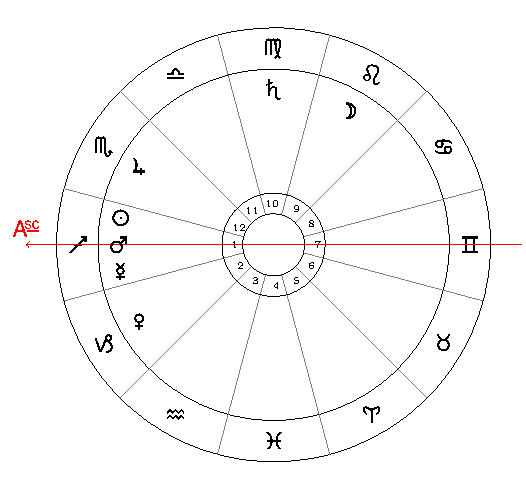
\includegraphics[width=.68\textwidth]{charts/5_11_1}
\caption{Chart 69 [V.11.1, GH L37]}
\label{fig:chart69}
\end{wrapfigure}

\noindent For example: \Sun, \Mars, \Mercury, Ascendant in \Sagittarius, \Moon\, in \Leo, \Saturn\, in \Virgo, \Jupiter\, in \Scorpio, \Venus\, in \Capricorn\footnote{\textit{Greek Horoscopes} dates the chart to December 15, 37 CE about sunrise}. 

The \Moon\, controls the second interval since it is two signs from \Saturn\footnote{The \Moon\, is two signs from \Saturn\, and transmits to him.}. The same is true of the \Sun, \Mars, \Mercury, and the Ascendant with respect to \Venus\footnote{Asc, \Sun, \Mars, \Mercury\, are two signs from \Venus\, and transmit to her.}. \Saturn, \Jupiter, and \Venus\, control the third interval\footnote{\Saturn\, is 3 signs from \Jupiter, \Jupiter\, is 3 signs from \Venus, \Venus\, is 3 signs from \Pisces, which is empty, in which case we look it's ruler, \Jupiter.}. \Saturn\, controls the fourth and fifth interval\footnote{\Saturn\, is 4 signs from the Asc, \Sun, \Mars, \Mercury, and 5 signs from \Venus. He appears to ignore that the \Moon\, is 4 from \Jupiter\, and 5 from the Asc, \Sun\, \Mercury\,and \Mars.}. The \Moon\, controls the sixth\footnote{The \Moon\, is 6  signs from \Venus.}. The seventh is common to all\footnote{The 7th place from every planet is empty.}. \Venus\, controls the eighth\footnote{\Venus\, hands off to the \Moon, 8 signs away.}. The \Sun, \Mars, \Mercury, and the Ascendant the ninth\footnote{The Asc, \Sun, \Mars\, and \Mercury\, hand off to the \Moon.}. \Jupiter\, the tenth and eleventh\footnote{Handing off to the \Moon\ in 10 signs, \Saturn\, in 11 signs.}, and \Venus\, the twelfth\footnote{Handing off to \Jupiter.}. 

The horoscope is in its 31st year. The operative stars and the critical points are found as follows: when calculating the previously mentioned critical points, begin at \textbf{/234K/} the third row (=third interval), because the preceding two intervals, the first and the second, are inoperative. (The first is operative to year 12, the second to year 24, the third to year 36, and so on.) 

It is calculated thus: since the 31st year falls in the eleventh column of the third interval\footnote{Schmidt says this is because 31 falls between the 10th and 11th interval of years i.e. it falls between (3x10) 30 and (3x11) 33 (VRS5 p51).}, and since \Saturn, \Jupiter, and \Venus\footnote{\tiny\Saturn\, hands off to \Jupiter, \Jupiter\, hands off to \Venus, and \Venus, hands off to \Pisces, an empty sign.  Schmidt suggests that using the age triad is an alternative to be used when a control planet (\Venus\, in this case) hands off to an empty sign (VRS5 p.51). The above table's use is as suggested by Schmidt (VRS5 p.49).} control the third interval at the nativity, investigate the stars \textbf{/223P/} in transit at the time in question to see if they transmit to another star or to themselves at a distance of 11 signs. 
\begin{mdframed}[backgroundcolor=cyan!5]
\fontsize{7}{7}\selectfont
Years that share the same 12 year intervals (subtract one to get actual age):
\vspace{-1em}
\begin{longtable}[c]{r|rrrrrrrrrrrr}
\hline
1st 	& 1	& 2	& 3	& 4	& 5	& 6 
		& 7	& 8	& 9	& 10	& 11	& 12 \\
2nd	& 13 & 14 & 15 & 16 & 17 & 18 
		& 19 & 20 & 21 & 22 & 23 & 24 \\
\rowcolor{red!10}3rd	& 25 & 26 & 26 & 28 & 29 & 30 
		& 31 & 32 & 33 & 34 & 35 & 36 \\ 
4th	& 37 & 38 & 39 & 40 & 41 & 42
		& 43 & 44 & 45 & 46 & 47 & 48 \\
5th 	& 49 & 50 & 51 & 52 & 53 & 54
		& 55 & 56 & 57 & 48 & 59 & 60 \\ 
6th	& 61 & 62 & 63 & 64 & 65 & 66 
		& 67 & 68 & 69 & 70 & 71 & 72 \\ 
7th	& 73 & 74 & 75 & 76 & 77 & 78
		& 79 & 80 & 81 & 82 & 83 & 84 \\
8th  & 85 & 86 & 87 & 88 & 89 & 90
		& 91 & 92 & 93 & 94 & 95 & 96 \\ \hline
\end{longtable}

Age Interval Years Based on Cycle Number
\vspace{-1em}
\begin{longtable}[c]{r|rrrrrrrrrrr}
\hline
1	& 2	& 3	& 4	& 5	& 6 	& 7	& 8	& 9	& 10	
	& \cellcolor{red!10}11	& 12 \\ \hline
2  & 4   	& 6 	& 8 	& 10 	& 12 	& 14 	& 16 	& 18 	& 20 	& 22 	& 24 \\
\rowcolor{red!10}3	& 6	& 9	& 12	& 15	& 18	& 21	& 24	
	& 27	& \cellcolor{yellow!20} 30	& \cellcolor{yellow!20} 33	& 26 \\
4	& 8	& 12	& 16	& 20	& 24	& 28	& 32	& 36	& 40	& 44	& 48 \\
5	& 10	& 15	& 20	& 25	& 30	& 35	& 40	& 45	& 50	& 55	& 60 \\
6	& 12	& 18	& 24	& 30	& 36	& 42	& 48	& 54	& 60	& 66	& 72 \\
7	& 14	& 21	& 28	& 35	& 42	& 49	& 56	& 63	& 70	& 77	& 84 \\
8	& 16	& 24	& 32	& 40	& 48	& 56	& 64	& 72	& 80	& 88	& 96 \\
9	& 18	& 27	& 36	& 45	& 54	& 63	& 72	& 81	& 90	& 99	& 108 \\
10 & 20 & 30 & 40 & 50 & 60 & 70 & 80 & 90 & 100 & 110 & 120 \\

\end{longtable}
\end{mdframed}
\newpage
{\fontsize{6}{6}\selectfont
\begin{longtable}[c]{|cc|c|c|c|c|c|c|c|c|c|c|c|c|}
\hline
 && \Aries & \Taurus & \Gemini & \Cancer & \Leo & \Virgo
 & \Libra &  \Scorpio & \Sagittarius & \Capricorn & \Aquarius & \Pisces 
 \\
\hline
&& & & &  &\Moon &\Saturn\cellcolor{green!10} & &\Jupiter\cellcolor{green!10} &\Mercury,\Sun,\Mars 
&\Venus\cellcolor{green!10} & &\\
\hline
\endhead
\Aries & & 1 & 12 & 11 & 10 & 9 & 8 & 7 & 6 & 5 & 4 	& 3 & 2 \\
\Taurus & & 2 & 1 & 12 & 11 & 10 & 9 & 8 & 7 & 6 & 5 & 4 & 3 \\
\rowcolor{red!10}
\Gemini & & 3 & 2 & 1 & 12 & 11 & 10 & 9 & 8 & 7 & 6 & 5 & 4 \\
\Cancer & & 4 & 3 & 2 & 1 & 12 & 11 & 10 & 9 & 8 & 7 & 6 & 5 \\
\Leo &\Moon & 5 & 4 & 3 & 2 & 1 & 12 & 11 & 10 & 9 & 8 & 7 & 6 \\
\Virgo &\Saturn
	& 6 & 5 & 4 & 3 & 2 & 1 & 12 & 11 & 10 & 9 & 8 & 7 \\
\Libra & & 7 & 6 & 5 & 4 & 3 & 2 & 1 & 12 & 11 & 10 & 9 & 8 \\
\Scorpio &\Jupiter\cellcolor{yellow!20}
	&  8 & 7 & 6 & 5 & 4 & 3\cellcolor{yellow!20} & 2 & 1 & 12 & 11 & 10 & 9 \\
\Sagittarius &\Mercury\Sun\Mars 
	& 9 & 8 & 7 & 6 & 5 & 4 & 3 & 2 & 1 & 12 & 11 & 10 \\
\Capricorn &\Venus\cellcolor{yellow!20} 
	& 10 & 9 & 8 & 7 & 6 & 5 & 4 & 3\cellcolor{yellow!20} & 2 & 1 & 12 & 11 \\
\Aquarius & & 11 & 10 & 9 & 8 & 7 & 6 & 5 & 4 & 3 & 2 & 1 & 12 \\
\Pisces & & 12 & 11 & 10 & 9 & 8 & 7 & 6 & 5 & 4 & 3\cellcolor{gray!20} & 2 & 1 \\
\hline
\caption{Critodemus' System for Example: 31st Year}
\end{longtable}
}

\begin{wrapfigure}[15]{r}{7cm}
\centering
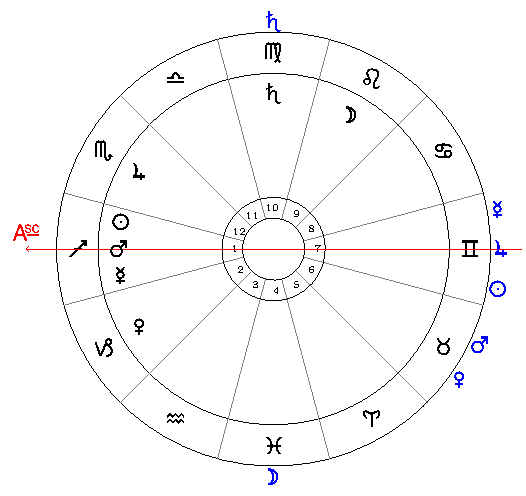
\includegraphics[width=.68\textwidth]{charts/5_11_1a}
\caption{\tiny Chart 69a [V.11.1, GH L37 Transits]}
\label{fig:chart69a}
\end{wrapfigure}

Take the preceding nativity: the stars’ positions at the time in question\footnote{i.e. take the planets transit positions at the time} were as follows: \Sun, \Jupiter, \Mercury\, in \Gemini, \Saturn\, in \Virgo, \Mars, \Venus\, in \Taurus, \Moon\, in \Pisces. 

\noindent Now the stars controlling the interval of 11 were \Saturn, \Jupiter, and \Venus\footnote{They are the same planets controlling the 3 sign interval; they also control the age interval (found earlier) of 11.} and we find at the time in question that \Venus\, has returned to a position 11 signs from the \Moon\footnote{The transit \Moon\, in \Pisces\, is 11 signs from transit \Venus\, in \Taurus.}, but that no star has returned to a position 11 signs from \Jupiter\footnote{\Aries, the 11th sign from transit \Jupiter\, in \Gemini, is empty.}. 

Immediately I move to the fourth row. I find 32 in the eighth position\footnote{The age interval for 32 would be 8 (4x8)}. None of the ruling stars are critical in the fourth interval\footnote{The \Moon\, hands off to \Jupiter\, in \Scorpio\, which is empty. \Saturn\, hands off to planets in the Ascendant which hand off to \Pisces, another empty sign. Presumably no transit planets were in their radix or age interval configurations.}. 
\newpage
{\fontsize{6}{6}\selectfont
\begin{longtable}[c]{|cc|c|c|c|c|c|c|c|c|c|c|c|c|}
\hline
 && \Aries & \Taurus & \Gemini & \Cancer & \Leo & \Virgo
 & \Libra &  \Scorpio & \Sagittarius & \Capricorn & \Aquarius & \Pisces 
 \\
\hline
&& & & &  &\Moon\cellcolor{green!10} &\Saturn\cellcolor{green!10} 
& &\Jupiter &\Mercury,\Sun,\Mars &\Venus & &\\
\hline
\endhead
\Aries & & 1 & 12 & 11 & 10 & 9 & 8 & 7 & 6 & 5 	
	& 4 	& 3 & 2 \\
\Taurus & & 2 & 1 & 12 & 11 & 10 & 9 & 8 & 7 & 6 & 5 & 4 & 3 \\
\Gemini & & 3 & 2 & 1 & 12 & 11 & 10 & 9 & 8 & 7 & 6 & 5 & 4 \\
\rowcolor{red!10}
\Cancer & & 4 & 3 & 2 & 1 & 12 & 11 & 10 & 9 & 8 & 7 & 6 & 5 \\
\Leo &\Moon & 5 & 4 & 3 & 2 & 1 & 12 & 11 & 10 & 9 & 8 & 7 & 6 \\
\Virgo &\Saturn
	& 6 & 5 & 4 & 3 & 2 & 1 & 12 & 11 & 10 & 9 & 8 & 7 \\
\Libra & & 7 & 6 & 5 & 4 & 3 & 2 & 1 & 12 & 11 & 10 & 9 & 8 \\
\Scorpio &\Jupiter\cellcolor{yellow!20}
	&  8 & 7 & 6 & 5 & 4\cellcolor{yellow!20} & 3 & 2 & 1 & 12 & 11 & 10 & 9 \\
\Sagittarius &\Mercury\Sun\Mars\cellcolor{yellow!20} 
	& 9 & 8 & 7 & 6 & 5 & 4\cellcolor{yellow!20} & 3 & 2 & 1 & 12 & 11 & 10 \\
\Capricorn &\Venus 
	& 10 & 9 & 8 & 7 & 6 & 5 & 4 & 3 & 2 & 1 & 12 & 11 \\
\Aquarius & & 11 & 10 & 9 & 8 & 7 & 6 & 5 & 4\cellcolor{gray!20} & 3 & 2 & 1 & 12 \\
\Pisces & & 12 & 11 & 10 & 9 & 8 & 7 & 6 & 5 & 4\cellcolor{gray!20} & 3 & 2 & 1 \\
\hline
\caption{Critodemus' System for Example: 32nd Year}
\end{longtable}
}

I move to the fifth interval \textsl{[33rd year]}: the \Moon\, and \Saturn\, are operative in the fifth interval and are found to be returning to each other five signs apart\footnote{Both the \Moon\, and \Saturn\, hand off to planets in the 5th interval. Maybe they have returned to their natal positions by transit?}.

{\fontsize{6}{6}\selectfont
\begin{longtable}[c]{|cc|c|c|c|c|c|c|c|c|c|c|c|c|}
\hline
 && \Aries & \Taurus & \Gemini & \Cancer & \Leo & \Virgo
 & \Libra &  \Scorpio & \Sagittarius & \Capricorn & \Aquarius & \Pisces 
 \\
\hline
&& & & &  &\Moon\cellcolor{green!10} &\Saturn\cellcolor{green!10} 
& &\Jupiter &\Mercury,\Sun,\Mars &\Venus & &\\
\hline
\endhead
\Aries & & 1 & 12 & 11 & 10 & 9 & 8 & 7 & 6 
	& \cellcolor{gray!20}5 & 4 & 3 & 2 \\
\Taurus & & 2 & 1 & 12 & 11 & 10 & 9 & 8 & 7 & 6 
	& \cellcolor{gray!20}5 & 4 & 3 \\
\Gemini & & 3 & 2 & 1 & 12 & 11 & 10 & 9 & 8 & 7 & 6 & 5 & 4 \\
\Cancer & & 4 & 3 & 2 & 1 & 12 & 11 & 10 & 9 & 8 & 7 & 6 & 5 \\
\rowcolor{red!10}
\Leo &\Moon & 5 & 4 & 3 & 2 & 1 & 12 & 11 & 10 & 9 & 8 & 7 & 6 \\
\Virgo &\Saturn
	& 6 & 5 & 4 & 3 & 2 & 1 & 12 & 11 & 10 & 9 & 8 & 7 \\
\Libra & & 7 & 6 & 5 & 4 & 3 & 2 & 1 & 12 & 11 & 10 & 9 & 8 \\
\Scorpio &\Jupiter 
	&  8 & 7 & 6 & 5 & 4 & 3 & 2 & 1 & 12 & 11 & 10 & 9 \\
\Sagittarius &\Mercury\Sun\Mars\cellcolor{yellow!20}
	& 9 & 8 & 7 & 6 & 5\cellcolor{yellow!20} & 4 & 3 & 2 & 1 & 12 & 11 & 10 \\
\Capricorn &\Venus\cellcolor{yellow!20} 
	& 10 & 9 & 8 & 7 & 6 & 5\cellcolor{yellow!20} & 4 & 3 & 2 & 1 & 12 & 11 \\
\Aquarius & & 11 & 10 & 9 & 8 & 7 & 6 & 5 & 4 & 3 & 2 & 1 & 12 \\
\Pisces & & 12 & 11 & 10 & 9 & 8 & 7 & 6 & 5 & 4 & 3 & 2 & 1 \\
\hline
\caption{Critodemus' System for Example: 33rd Year}
\end{longtable}
}

I move to the sixth interval \textsl{[34th year]}: no stars are six signs apart\footnote{No transit planets 6 signs apart? The \Moon\, and \Venus\, are 6 signs apart in the radix.}. 

I move to the row of the seventh interval \textsl{[35th year]}. [The chronocratorship is found to be passing through the fifth interval\footnote{The age interval 7th row has 35 under the 5th column}.] The seventh interval is found to be empty of any star (as mentioned above)\footnote{No planets are 7 signs apart in the radix.}; \Mars\, and \Venus\, to \Saturn\, <?>. 

I move to the row of the eighth interval \textsl{[36th year]}: \Venus\, rules the eighth interval because of the factor 4. It is returning to no star\footnote{\Venus\, in a 4 year hands over to \Aries, which is empty; however, she also hands over to the \Moon\, in an 8 year which Valens seems to be ignoring.}. 

Then to the critical point of the ninth interval \textsl{[37th year]}: the \Sun, \Mars, \Mercury, the Ascendant, and \Venus\, rule the ninth interval; 36 is in this row\footnote{\Venus, in a 9th intervals hands off to \Saturn\, and \Mercury,\Sun\, and \Mars\, hand off to the \Moon. In the Age Interval 9th row, 36 is under the 4th column (9x4=36)}.

At a 4-year interval the \Sun, \Jupiter, and \Mercury\, are found to be returning to \Saturn\footnote{Possibly an error in the original text, see end of next paragraph, this line appears to repeat it.}. 

Next I move to the tenth interval \textsl{[38th year]}: the \Sun,\Mars, \Mercury, \Jupiter, and the Ascendant rule the tenth; in this row is the number 4; therefore the \Sun, \Mercury, and \Jupiter\, are found to be transmitting to \Saturn\footnote{The \Sun,\Mercury\, and \Mars\, are transmitting to \Saturn, \Jupiter\, is transmitting to the \Moon.}.

{\fontsize{6}{6}\selectfont
\begin{longtable}[c]{|cc|c|c|c|c|c|c|c|c|c|c|c|c|}
\hline
 && \Aries & \Taurus & \Gemini & \Cancer & \Leo & \Virgo
 & \Libra &  \Scorpio & \Sagittarius & \Capricorn & \Aquarius & \Pisces 
 \\
\hline
&& & & &  &\Moon &\Saturn
& &\Jupiter\cellcolor{green!10} &\Mercury,\Sun,\Mars\cellcolor{green!10} &\Venus & &\\
\hline
\endhead
\Aries & & 1 & 12 & 11 & 10 & 9 & 8 & 7 & 6 & 5 & 4 & 3 & 2 \\
\Taurus & & 2 & 1 & 12 & 11 & 10 & 9 & 8 & 7 & 6 & 5 & 4 & 3 \\
\Gemini & & 3 & 2 & 1 & 12 & 11 & 10 & 9 & 8 & 7 & 6 & 5 & 4 \\
\Cancer & & 4 & 3 & 2 & 1 & 12 & 11 & 10 & 9 & 8 & 7 & 6 & 5 \\
\Leo &\Moon\cellcolor{yellow!20} & 5 & 4 & 3 & 2 & 1 & 12 & 11 & 10\cellcolor{yellow!20} & 9 & 8 & 7 & 6 \\
\Virgo &\Saturn\cellcolor{yellow!20}
	& 6 & 5 & 4 & 3 & 2 & 1 & 12 & 11 
	& 10\cellcolor{yellow!20} & 9 & 8 & 7 \\
\Libra & & 7 & 6 & 5 & 4 & 3 & 2 & 1 & 12 & 11 & 10 & 9 & 8 \\
\Scorpio &\Jupiter 
	&  8 & 7 & 6 & 5 & 4 & 3 & 2 & 1 & 12 & 11 & 10 & 9 \\
\Sagittarius &\Mercury\Sun\Mars 
	& 9 & 8 & 7 & 6 & 5 & 4 & 3 & 2 & 1 & 12 & 11 & 10 \\
\rowcolor{red!10}
\Capricorn &\Venus 
	& 10 & 9 & 8 & 7 & 6 & 5 & 4 & 3 & 2 & 1 & 12 & 11 \\
\Aquarius & & 11 & 10 & 9 & 8 & 7 & 6 & 5 & 4 & 3 & 2 & 1 & 12 \\
\Pisces & & 12 & 11 & 10 & 9 & 8 & 7 & 6 & 5 & 4 & 3 & 2 & 1 \\
\hline
\caption{Critodemus' System for Example: 38th Year}
\end{longtable}
}


The \mndl chronocrators found by using these intervals will be incontrovertibly active and operative when their rulers at the nativity have the same intervals in their transits at the time in question as they had at the nativity.
\newpage